\documentclass{beamer}

%% \documentclass[handout]{beamer}
%% % use this with the [handout] option to create handouts for the audience
%% \usepackage{pgfpages}
%% \pgfpagesuselayout{2 on 1}[a4paper,border shrink=5mm]

\mode<presentation>
{
  \usetheme{Diku}
% set this to your preferences:
  \setbeamercovered{invisible}
%  \setbeamercovered{transparent}
}

\usepackage{graphicx}
\usepackage{epic}

\usepackage{amsmath}
\usepackage{amssymb}
\usepackage{amsthm}

\newcommand{\basetop}[1]{\vtop{\vskip-1ex\hbox{#1}}}
\newcommand{\source}[1]{\let\thefootnote\relax\footnotetext{\scriptsize\textcolor{kugray1}{Source: #1}}}

% for coloured code citation in text:
\usepackage{fancyvrb}

%%%%%%%%%%%%%%%%%%%%%%%%%%%%%%%%%
%%%%%    code sections   %%%%%%%%
%%%%%%%%%%%%%%%%%%%%%%%%%%%%%%%%%

% code highlighting commands in own block
\DefineVerbatimEnvironment{code}{Verbatim}{fontsize=\scriptsize}
\DefineVerbatimEnvironment{icode}{Verbatim}{fontsize=\scriptsize}

% Fancy code with color commands:
\DefineVerbatimEnvironment{colorcode}%
        {Verbatim}{fontsize=\scriptsize,commandchars=\\\{\}}

%%%%%%%%%%%%%%%%%%%%%%%%%%%%%%%%%%
%%%%%    some coloring    %%%%%%%%

\definecolor{Red}{RGB}{220,50,10}
\definecolor{Blue}{RGB}{0,51,102}
\definecolor{Yellow}{RGB}{102,51,0}
\definecolor{Orange}{RGB}{178,36,36}
\definecolor{Grey}{RGB}{180,180,180}
\definecolor{Green}{RGB}{20,120,20}
\definecolor{Purple}{RGB}{160,50,100}
\newcommand{\red}[1]{\textcolor{Red}{{#1}}}
\newcommand{\blue}[1]{\textcolor{Blue}{{#1}}}
\newcommand{\yellow}[1]{\textcolor{Yellow}{{#1}}}
\newcommand{\orange}[1]{\textcolor{Orange}{{#1}}}
\newcommand{\grey}[1]{\textcolor{Grey}{{#1}}}
\newcommand{\green}[1]{\textcolor{Green}{{#1}}}
\newcommand{\purple}[1]{\textcolor{Purple}{{#1}}}




% use "DIKU green" from our color theme for \emph
\renewcommand{\emph}[1]{\textcolor{structure}{#1}}
% use some not-too-bright red for an \emp command
\definecolor{DikuRed}{RGB}{130,50,32}
\newcommand{\emp}[1]{\textcolor{DikuRed}{ #1}}
\definecolor{CosGreen}{RGB}{10,100,70}
\newcommand{\emphh}[1]{\textcolor{CosGreen}{ #1}}
\definecolor{CosBlue}{RGB}{55,111,122}
\newcommand{\emphb}[1]{\textcolor{CosBlue}{ #1}}
\definecolor{CosRed}{RGB}{253,1,1}
\newcommand{\empr}[1]{\textcolor{CosRed}{ #1}}

\newcommand{\mymath}[1]{$ #1 $}
\newcommand{\myindx}[1]{_{#1}}
\newcommand{\myindu}[1]{^{#1}}

\newcommand{\Fasto}{\textsc{Fasto}\xspace}


%%%%%%%%%%%%%%%%%%%%

\title[Interpretation]{Interpretation}

\author[C.~Oancea]{Cosmin E. Oancea\\{\tt cosmin.oancea@diku.dk}}

\institute{Department of Computer Science (DIKU)\\University of Copenhagen}


\date[December 2012]{December 2012 Compiler Lecture Notes}


\begin{document}

\titleslide

\input{Struct_Interm/StructInterpr}

\begin{frame}[fragile]
	\tableofcontents
\end{frame}


%%%%%%%%%%%%%%%%%%%%%%%%%%%%%%%%%%%%%%%%%%%%%%%%%%%%%%%%%%%%%%%%%%%%%%
\section{\textsc{Fasto} Language Semantics}


\begin{frame}[fragile,t]
\frametitle{\textsc{Fasto} Language: Function Declaration and Types}



%\begin{block}{Optimize Parallelism Via Serial Chunking: Compiler's Job}
\begin{columns}
\column{0.6\textwidth}
\renewcommand{\arraystretch}{0.85}
\[\begin{array}{lcl}
Program & \rightarrow & Funs \\[2ex]

Funs & \rightarrow & Fun \\
Funs & \rightarrow & Fun~Funs \\[2ex]

Fun & \rightarrow & Type {\bf id}~(~TypeIds~)~\mbox{\tt =}~Exp \\[2ex]

TypeIds & \rightarrow & Type~{\bf id}           \\
TypeIds & \rightarrow & Type~{\bf id}~,~TypeIds \\[2ex]  

Type & \rightarrow & \mbox{\tt int}  \\
Type & \rightarrow & \mbox{\tt char} \\
Type & \rightarrow & \mbox{\tt bool} \\
Type & \rightarrow & {\tt [} Type {\tt ]} \\[2ex]

Exps & \rightarrow & Exp \\
Exps & \rightarrow & Exp~\mbox{\tt ,}~Exps
\end{array}\]

\column{0.38\textwidth}
\begin{itemize}
    \item First-order functional language \& mutually recursive functions.
    \item Program starts by executing ``main'', which takes no args.
    \item Separate namespaces for vars \& funs.
    \item Illegal for two formal params of the same function to share the same name.
    \item Illegal for two functions to share the same name.
\end{itemize}
\end{columns}
%\end{block}


\end{frame}


\begin{frame}[fragile,t]
\frametitle{\textsc{Fasto} Language: Basic Expressions}

\begin{columns}
\column{0.6\textwidth}
\renewcommand{\arraystretch}{0.85}
\[\begin{array}{lcl}
Exp & \rightarrow & \mbox{\bf id} \\
Exp & \rightarrow & \mbox{\bf num} \\
Exp & \rightarrow & \mbox{\bf charlit} \\[2ex]

Exp & \rightarrow & Exp~\mbox{\tt +}~ Exp \\
Exp & \rightarrow & Exp~\mbox{\tt -}~ Exp \\
Exp & \rightarrow & Exp~\mbox{\tt <}~ Exp \\
Exp & \rightarrow & Exp~\mbox{\tt =}~ Exp \\[2ex]

Exp & \rightarrow & \mbox{\tt if}~Exp~\mbox{\tt then}~ Exp~\mbox{\tt else}~Exp\\[1ex]

Exp & \rightarrow & \mbox{\tt let}~\mbox{\bf id}~\mbox{\tt =}~Exp~\mbox{\tt in}~Exp \\[1ex]

Exp & \rightarrow & \mbox{\bf id}~() \\
Exp & \rightarrow & \mbox{\bf id}~(~Exps~) \\

\end{array}\]

\column{0.38\textwidth}
\begin{itemize}
    \item {\tt +}, {\tt -} defined on ints.
    \item {\tt =}, {\tt <} defined on basic-type values.
    \item Static Scoping: {\tt let} bindings and function declarations create new scopes.
    \item A {\tt let id ...} may hide an outer-scope var also named {\tt id}.
    \item Call by Value.
\end{itemize}
\end{columns}

\end{frame}



\begin{frame}[fragile,t]
\frametitle{Demonstrating Recursive Calls and IO in Fasto}

%[fontsize=\scriptsize]
\begin{block}{Fibonacci Example and Use of Read/Write}
\begin{colorcode}
fun \emphh{int fibo(int n)} = if        (n = 0) then 1
                        else if (n = 1) then 1
                        else \emphh{fibo(n-1)} + \emphh{fibo(n-2)}

fun int main () = let w = \emp{write}("Enter Fibonacci's number: \textbackslash n")
                  in  let n = \emp{read(int)}
                      in let w = \emp{write}("Result is: \textbackslash n")
                         in let ww = \emp{write}(w)  //what is printed?
                             in \emp{write}( \emphh{fibo(n)} )
\end{colorcode} 
\end{block}

\pause

{\em Polymorphic Functions} {\tt read} and {\tt write}:\smallskip
\begin{itemize}
    \item the only constructs in \textsc{Fasto} exhibiting side-effects (IO).\smallskip
    \item valid uses of {\tt read}: {\tt read(int)}, {\tt read(char)},
            or {\tt read(bool)};
          takes a type parameter and returns a (read-in) value of that type.\smallskip
    \item {\tt write : }$\alpha \rightarrow \alpha$, where $\alpha$ can be 
            {\tt int}, {\tt char}, {\tt bool}, {\tt [char]}, or {\bf stringlit}.
            \emp{{\tt write} {\em returns (a copy of) its input parameter.}}
\end{itemize}

\end{frame}



\begin{frame}[fragile,t]
\frametitle{\textsc{Fasto} Language: Array Constructors \& Combinators}

\begin{columns}
\column{0.6\textwidth}
\renewcommand{\arraystretch}{0.85}
\[\begin{array}{lcl}
Exp & \rightarrow & \mbox{\tt read~(}~Type~\mbox{)} \\[.5ex]
Exp & \rightarrow & \mbox{\tt write~(}~Exp~\mbox{)} \\[2ex]

Exp & \rightarrow & \mbox{\bf stringlit} \\ [.5ex]
Exp & \rightarrow & \mbox{\tt \{}~Exps~\mbox{\tt \}}\\[.5ex]
Exp & \rightarrow & \mbox{\tt iota~(}~Exp~\mbox{)} \\[.5ex]
Exp & \rightarrow & \mbox{\tt replicate~(}~Exp~{\tt ,}~Exp~\mbox{)} \\[2ex]

Exp & \rightarrow & \mbox{\tt map~(}~{\bf id}~{\tt ,}~Exp~\mbox{)} \\[.5ex]
Exp & \rightarrow & \mbox{\tt reduce~(}~{\bf id}~{\tt ,}~Exp~{\tt ,}~Exp~\mbox{)} \\[2ex]

Exp & \rightarrow & \mbox{\bf id}~{\tt [}~Exp~{\tt ]} \\
\end{array}\]

\column{0.38\textwidth}
\begin{itemize}
    \item {\tt read} / {\tt write} polymorphic operators,
    \item array constructors: string and array literals, {\tt iota}, {\tt replicate},
    \item second-order array combinators (\textsc{soac}): {\tt map} and {\tt reduce},
    \item array indexing: check if index is within bounds.
\end{itemize}
\end{columns}

\end{frame}


\begin{frame}[fragile,t]
\frametitle{\textsc{Fasto}'s Array Constructors \& Combinators}

Array Constructors:
\begin{itemize}
    \item literals: \emph{{\tt \{~\{1+2, x+1, x+y\}, \{5, ord('e')\}~\}}}\emp{{\tt~:~[[int]]}}
    \item {\bf stringlit}: \emph{{\tt "Hello"~$\equiv$~\{'H','e','l','l','o'\}}}\emp{{\tt~:~[[int]]}}\pause
    \item {\tt iota(n)~$\equiv$}~\emph{{\tt\{0,1,2,...,n-1\}}}; {\em type of} 
        \emp{{\tt iota~:~int~$\rightarrow$~[int]}}\pause
    \item {\tt replicate(n, q)~$\equiv$}~\emph{{\tt\{q, q, ..., q\}}}, i.e., an array of size {\tt n},\\
          {\em type of} \emp{{\tt{}replicate : int * $\alpha~\rightarrow~$[$\alpha$]}}.\\
        What is the result of {\tt replicate(2, \{8, 9\})} ?
\end{itemize}

\pause
\bigskip

Second-Order Array Combinators:
\begin{itemize}
    \item {\tt map(f, \{x$_1$, .., x$_n$\}) = \emph{\{f(x$_1$, .., f(x$_n$))\}}}, where 
        type of \emp{{\tt{}x$_i$~:~$\alpha$}}, of 
        \emp{{\tt f~:~$\alpha\rightarrow\beta$}}, of
        \emp{{\tt map~:~($\alpha\rightarrow\beta$)~*~[$\alpha$]$~\rightarrow$~[$\beta$]}}
        \pause
    \item {\tt reduce($\odot$,~e,~\{x$_1$,x$_2$,..,x$_n$\})~=~\emph{(..(e$\odot$x$_1$)..$\odot$x$_n$)}}, where 
        type of \emp{{\tt{}x$_i$~:~$\alpha$}}, of \emp{{\tt{}e~:~$\alpha$}}, 
        type of \emp{{\tt{}$\odot$~:~$\alpha$~*~$\alpha$~$\rightarrow$~$\alpha$}}\\
        type of \emp{{\tt reduce~:~($\alpha$~*~$\alpha$~$\rightarrow$~$\alpha$)~*~$\alpha$~*~[$\alpha$]~$\rightarrow$~$\alpha$}}.
\end{itemize}

\end{frame}



\begin{frame}[fragile,t]
\frametitle{Demonstrating Map-Reduce Programming}

%[fontsize=\scriptsize]
\begin{block}{Can We Write Main Using Map and Reduce?}
\begin{colorcode}
\emp{foldl : \mymath{(\alpha * \beta \rightarrow \beta) * \beta * [\alpha] \rightarrow \beta}}
\emp{foldl(\mymath{\odot}, e, \{x\mymath{\myindx{1}}, .., x\mymath{\myindx{n}}\}) \mymath{\equiv} (x\mymath{\myindx{n} \odot} .. (x\mymath{\myindx{1} \odot} e) ..)}

fun bool f(int a, bool b) = (a > 0) && b
fun bool main() = let x = \{1, 2, 3\}
                  in \emp{foldl(f, True, x)}

\end{colorcode} 
\end{block}

\end{frame}


\begin{frame}[fragile,t]
\frametitle{Demonstrating Map-Reduce Programming}

%[fontsize=\scriptsize]
\begin{block}{Why Doe Fasto {\em Not} Support Foldl?}
\begin{colorcode}
\emp{foldl : \mymath{(\alpha * \beta \rightarrow \beta) * \beta * [\alpha] \rightarrow \beta}}
\emp{foldl(\mymath{\odot}, e, \{x\mymath{\myindx{1}}, .., x\mymath{\myindx{n}}\}) \mymath{\equiv} (x\mymath{\myindx{n} \odot} .. (x\mymath{\myindx{1} \odot} e) ..)}

fun bool f(int a, bool b) = (a > 0) && b
fun bool main() = let x = \{1, 2, 3\}
                  in \emp{foldl(f, True, x)}

\end{colorcode} 
\end{block}


\begin{block}{Because It Is Typically The Composition of a Map With a Reduce:}
\begin{colorcode}
\emphh{map :    \mymath{(\alpha \rightarrow \beta) * [\alpha] \rightarrow [\beta]}}
\emphh{map      (f,    \{x\mymath{\myindx{1}}, .., x\mymath{\myindx{n}}\}) \mymath{\equiv} \{f(x\mymath{\myindx{1}}, .., f(x\mymath{\myindx{1}}))\}}

\emp{reduce : \mymath{(\alpha * \alpha \rightarrow \alpha) * \alpha * [\alpha] \rightarrow \alpha}}
\emp{reduce   (\mymath{\odot}, e, \{x\mymath{\myindx{1}}, .., x\mymath{\myindx{n}}\}) \mymath{\equiv} (x\mymath{\myindx{n} \odot} .. (x\mymath{\myindx{1} \odot} e) ..)}

fun bool f(int a) = a > 0
fun bool main() = let x = \{1, 2, 3\} in
                  let \emphh{y = map(f, x)}                  
                  in \emp{reduce}(op &&, True, \emphh{y})

\end{colorcode} 
\end{block}

\end{frame}


\begin{frame}[fragile,t]
\frametitle{Array Combinators \& Read and Write}

\begin{block}{What Is Printed If The User Types in: ``1 2 8 9''?}
\begin{colorcode}
fun  int writeInt   ( int i ) = write(i)
fun  int  readInt   ( int i ) = read(int)
fun [int] readIntArr( int n ) = map( readInt, iota(n) )

fun [int] plusV2([int] a, [int] b) = \{ a[0]+b[0], a[1]+b[1] \}

fun [int] main() = let arr2 = \emphh{map(readIntArr, replicate(2,2))} in
                   let arr1 = \emp{reduce(plusV2, \{0,0\}, arr2)}     in
                       map( writeInt, arr1 )  
\end{colorcode} 
\end{block}
\smallskip
\pause
\emph{{\tt readIntArr(n)}} ``reads'' a $1D$ array of $n$ elements.

\bigskip

\emphh{{\tt map(readIntArr,replicate(2,2))}} $\equiv$ 
{\tt map(readIntArr,{2,2})}$\equiv$\\
    {\tt \{readIntArr(2),readIntArr(2)\}} builds $2D$ array {\tt \{\{1,2\},\{8,9\}\}}.
\end{frame}



\begin{frame}[fragile,t]
\frametitle{Array Combinators \& Read and Write}

\begin{block}{What Is Printed If The User Types in: ``1 2 8 9''?}
\begin{colorcode}
fun  int writeInt   ( int i ) = write(i)
fun  int  readInt   ( int i ) = read(int)
fun [int] readIntArr( int n ) = map( readInt, iota(n) )

fun [int] plusV2([int] a, [int] b) = \{ a[0]+b[0], a[1]+b[1] \}

fun [int] main() = let arr2 = \emphh{map(readIntArr, replicate(2,2))} in
                   let arr1 = \emp{reduce(plusV2, \{0,0\}, arr2)}     in
                       map( writeInt, arr1 )  
\end{colorcode} 
\end{block}

\smallskip

So, \emphh{{\tt map(readIntArr,replicate(2,2))}} $\equiv$ {\tt \{\{1,2\},\{8,9\}\}}.
  
\bigskip

\emp{{\tt reduce( plusV2, \{0,0\}, \{\{1,2\},\{8,9\}\} )}} $\equiv$ \\
\pause
{\tt plusV2( plusV2(\{0,0\}, \{1,2\}), \{8,9\} )} $\equiv$\\
{\tt plusV2( \{0+1,0+2\}, \{8,9\} )} $\equiv$ {\tt \{1+8, 2+9\}} $\equiv$ {\tt \{9,11\}}.

\bigskip

Finally, \emph{{\tt map(writeInt,arr1)}} prints the elements of {\tt arr1}, 
i.e., {\tt 9 11}!
\end{frame}

%%%%%%%%%%%%%%%%%%%%%%%%%%%%%%%%%%%%%%%%%%%%%%%%%%%%%%%%%%%%%%%%%%%%%%
\section{Interpretation: Intuition and Symbol Tables}

\begin{frame}[fragile]
	\tableofcontents[currentsection]
\end{frame}

\begin{frame}[fragile,t]
   \frametitle{Interpretation Intuition: Solving First-Grade Math}

\begin{block}{$~~~~~~~~~~$Term Rewriting $~~~~~~~~~~${\em vs.}$~~~~~~~~~~$ Interpretation}
\begin{columns}
\column{0.50\textwidth}
\begin{colorcode}[fontsize=\scriptsize]
q = (7 + 5) / 3 + (7 + 8) / 5
  = 12 / 3      + (7 + 8) / 5
  = 4           + (7 + 8) / 5
  = 4           + 15 / 5
  = 4           + 3

  = 7
\end{colorcode} 
\column{0.4\textwidth}
\begin{colorcode}[fontsize=\scriptsize]
x  = 7 + 5     ( = 12 )
y\mymath{\myindx{1}} = x / 3     ( = 12 / 3 = 4)

x  = 7 + 8     ( = 12)
y\mymath{\myindx{2}} = x / 5     ( = 15 / 5 = 3)

q  = y\mymath{\myindx{1}} + y\mymath{\myindx{2}}   ( = 4 + 3 = 7 ) 
\end{colorcode}
\end{columns}
\end{block}

\pause

\begin{block}{$~~~~~$Let (Partial) Semantics $~~~~~~~~~~~~~~~~~$ Program to evaluate {\tt q}}
\begin{columns}
\column{0.4\textwidth}
{\tt let t = e$_1$ in e$_2$} 

\smallskip

{\em \emph{Semantics:} evaluate {\tt e$_1$},}\\
{\em replace {\tt t} with {\tt e$_1$}'s value}\\
{\em in {\tt e$_2$}, and evaluate {\tt e$_2$}}
\column{0.5\textwidth}
\begin{colorcode}[fontsize=\small]
let x = 7 + 5
in  let y\mymath{\myindx{1}} = x / 3
    in  let x = 7 + 8
        in  let y\mymath{\myindx{2}} = x / 5
            in  y\mymath{\myindx{1}} + y\mymath{\myindx{2}}
\end{colorcode}
\end{columns}
\end{block}


\end{frame}


\begin{frame}[fragile,t]
   \frametitle{How to Interpret? Lang. Semantics + Symbol Table}

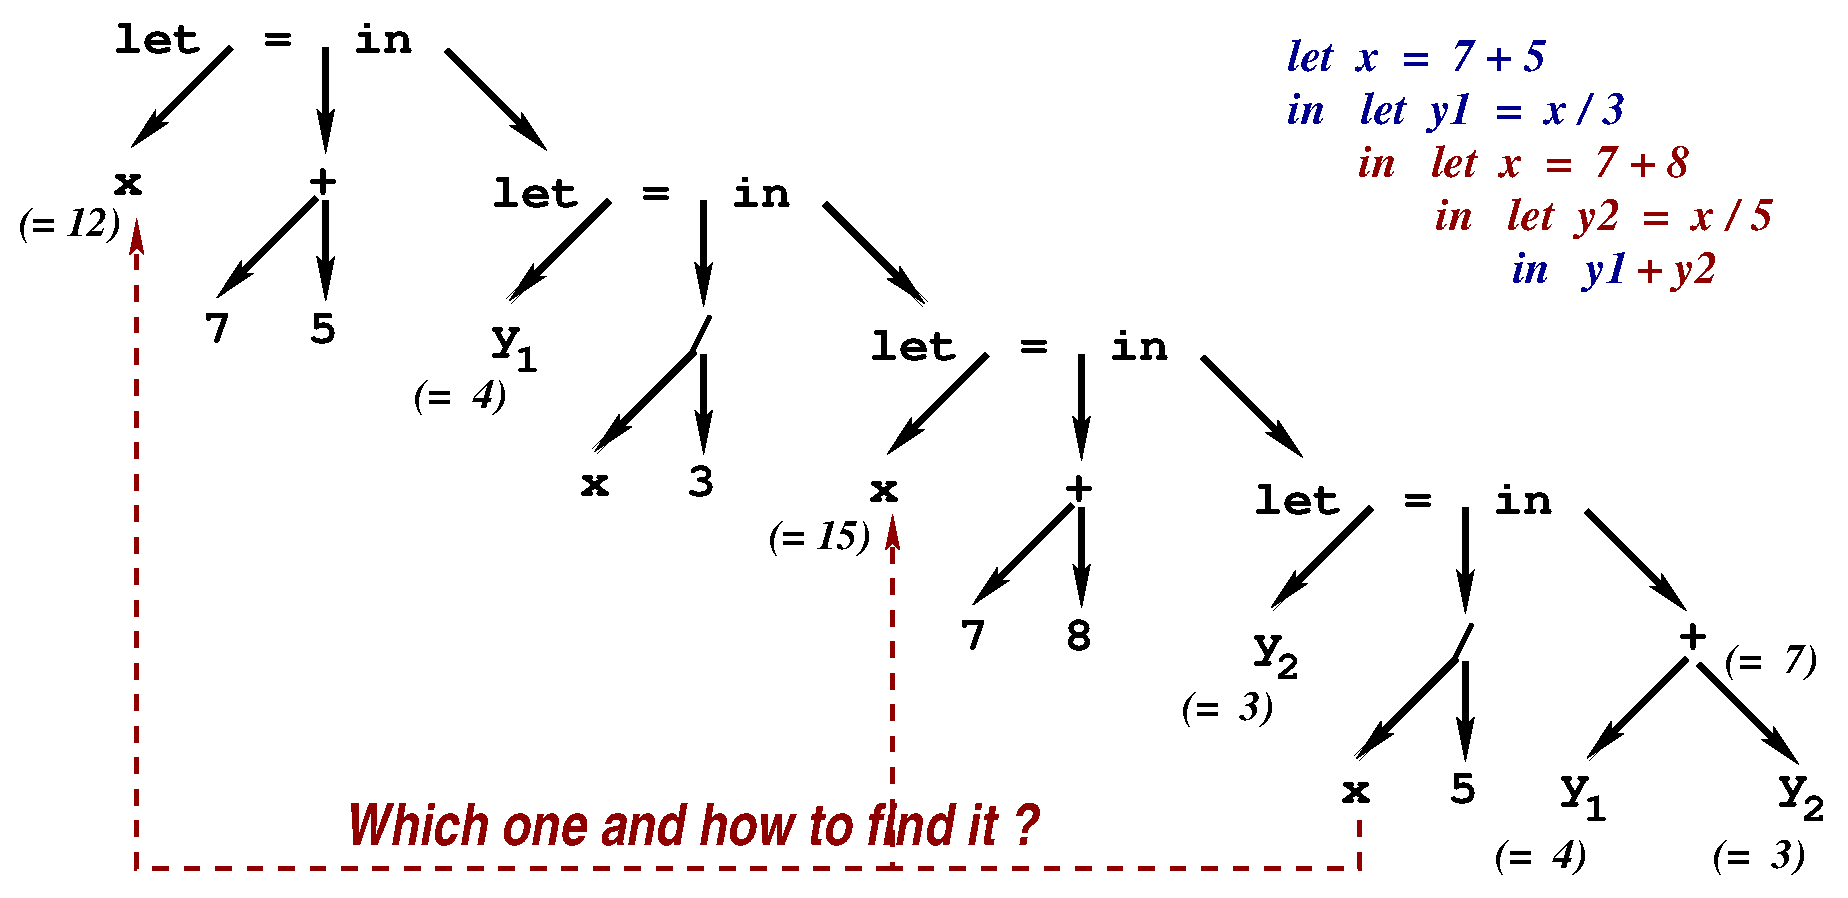
\includegraphics[width=67ex]{Figures/ExpIntNoStack}

\bigskip

{\em Semantics:} The use of {\tt x} refers to which of the two variables named {\tt x}?

\bigskip

{\em Symbol Table:} How to keep track of the values of various variables?


\end{frame}


\begin{frame}[fragile,t]
   \frametitle{How to Interpret? Lang. Semantics + Symbol Table}

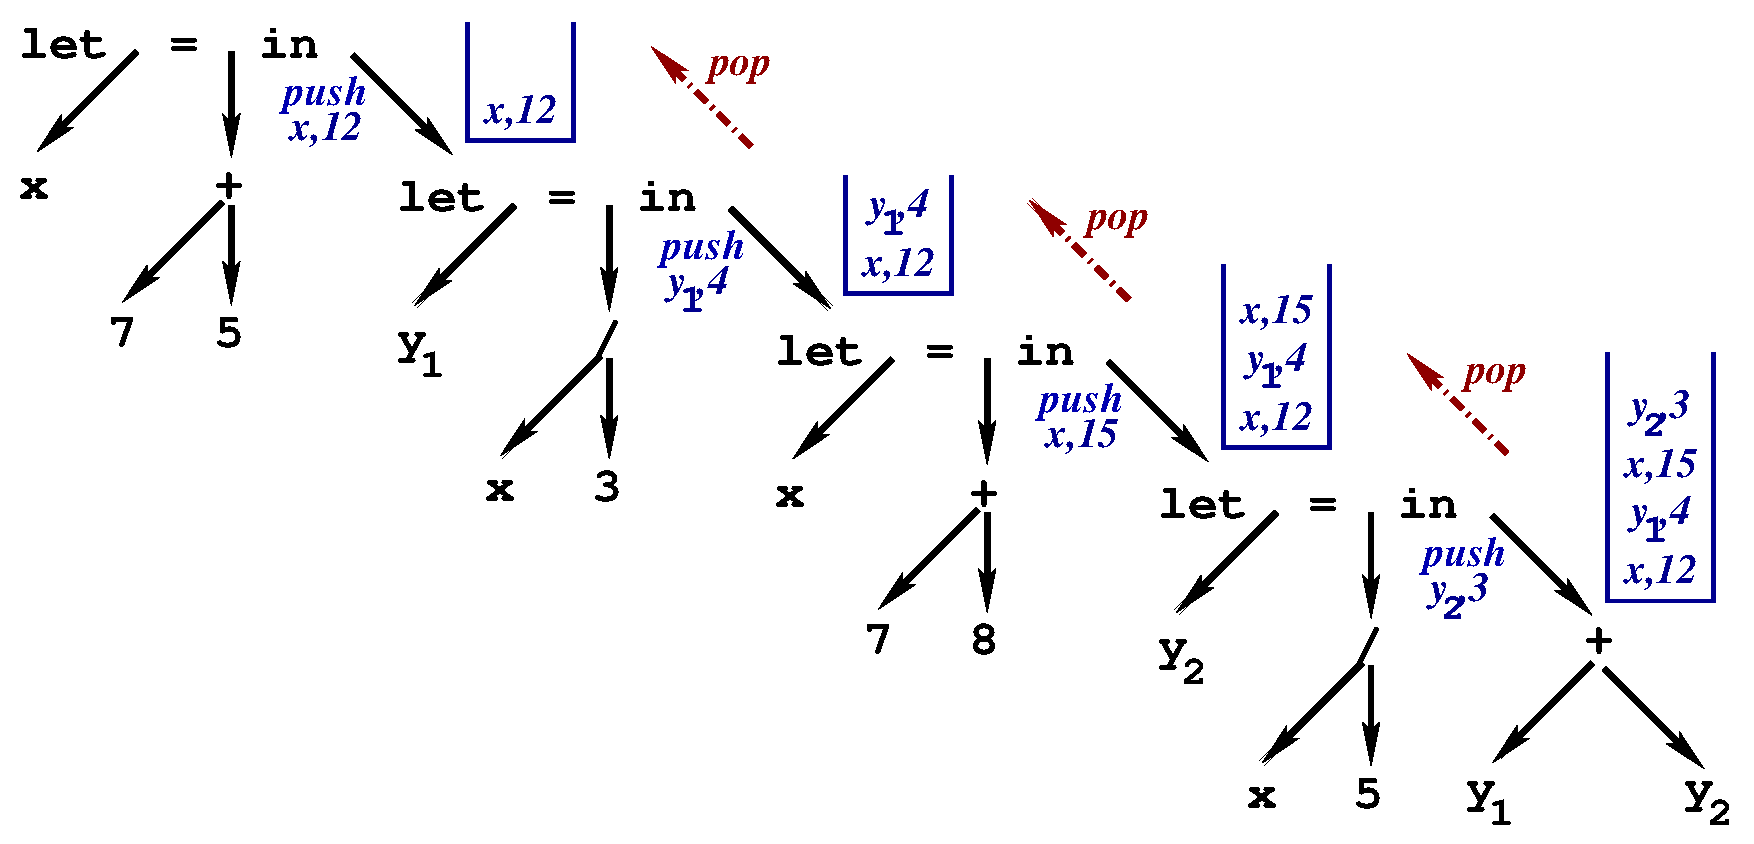
\includegraphics[width=65ex]{Figures/ExpIntStack}

\bigskip

{\em Semantics:} The use of {\tt x} refers to the ``closest''-outer scope that provides a definition for {\tt x}.

\bigskip

{\em Symbol Table:} the implementation uses a stack, which is scanned top down and returns the first encountered binding of {\tt x}.


\end{frame}


\begin{frame}[fragile,t]
   \frametitle{Symbol Table}

\emp{{\em Symbol Table:}} binds names to associated information.

\emp{Operations:}
\begin{itemize}
    \item \emph{\em empty:} empty table, i.e., no name is defined.\smallskip
    \item \emph{\em bind:} records a new {\tt (name,info)} association. If {\tt name}
        already in the table, the new binding takes precedence.\smallskip
    \item \emph{\em look-up:} finds the information associated to a name.
        The result must indicate also whether the name was present in the table.\smallskip
    \item \emph{\em enter}s a new scope: semantically adds new bindings.\smallskip
    \item \emph{\em exit}s a scope: restores the table to what it has been before
                    entering the current scope.
\end{itemize} 

\bigskip

\alert{For Interpretation: what is the info associated with a named variable?}

\end{frame}




\begin{frame}[fragile,t]
   \frametitle{Symbol Table}

\emp{Easiest implementation is a stack:} (i) \emph{\em bind} pushes a new binding, 
(ii) \emph{\em lookup} searches the stack top down, 
(iii) \emph{\em enter} pushes a marker,
(iv) \emph{\em exit} pops all elements up-to-and-including the first marker. 
\alert{Example!}

\begin{block}{Implementation in a Functional Language }
\begin{columns}
\column{0.50\textwidth}
\begin{colorcode}[fontsize=\scriptsize]
fun empty() = []

fun bind n i stab = (n,i)::stab
\end{colorcode} 
\column{0.4\textwidth}
\begin{colorcode}[fontsize=\scriptsize]
fun lookup n []      = NONE
  | lookup n ((n1,i1)::tab) =
      if  (n=n1) then SOME i1
      else lookup n tab 
\end{colorcode}
\end{columns}
\end{block}

Functional Implementation uses a list:
\begin{itemize}
    \item \emph{\em enter} saves the reference of the current (old)
        table, and creates a new table by appending new bindings to 
        the current symbol table.
    \item \emph{\em exit} discards the current table and uses the old table 
            (previously saved in enter).
\end{itemize}

\end{frame}

%%%%%%%%%%%%%%%%%%%%%%%%%%%%%%%%%%%%%%%%%%%%%%%%%%%%%%%%%%%%%%%%%%%%%%%
\section{Interpretation: Problem Statement and Notations}

\begin{frame}[fragile]
	\tableofcontents[currentsection]
\end{frame}


\begin{frame}[fragile,t]
   \frametitle{What is Interpretation?}

\begin{block}{$~~~~~~~~~~~~~$ Compiler $~~~~~~~~~~~~~$ {\em vs.} $~~~~~~~~~~~~~~$ Interpreter}
\begin{columns}
\column{0.31\textwidth}
\begin{tabular}{c}
{\em source program}\\
$\downarrow$\\
\framebox{\emph{Compiler}}\\
$\downarrow$\\
{\em target program}
\end{tabular}
\column{0.31\textwidth}
\begin{tabular}{c}
{\em input}\\
$\downarrow$\\
\framebox{Target Program}\\
$\downarrow$\\
{\em output}
\end{tabular}
\column{0.31\textwidth}
\begin{tabular}{c}
{\em source}$~~~~~~~~~~~$\\
{\em program}$~~~${\em input}\\
$\downarrow~~~~~~~\downarrow$\\
\framebox{\emp{Interpreter}}\\
$\downarrow$\\
{\em output}
\end{tabular}
\end{columns}
\end{block}

{\em The interpreter} directly {\em executes} one by one the operations specified
in the {\em source program} on the {\em input} supplied by the user, by using the
facilities of its implementation language.

\bigskip

{\em Why interpret?} Debugging, Prototype-Language Implementation, etc.

\end{frame}


\begin{frame}[fragile,t]
   \frametitle{Notations Used for Interpretation}

We logically split the abstract-syntax representation (\textsc{AbSyn}) into
different {\em syntactic categories}: expressions, function decl, etc.

\bigskip

Implementing the interpreter $\equiv$ implementing each syntactic category
via a function, that uses case analysis of \textsc{AbSyn}-type constructors.

\bigskip

In practice we work on \textsc{AbSyn}, but here we represent interpretation
generically by using a notation that resembles the language grammar.

\bigskip

For symbols representing names, numbers, and the like, we use special
functions that return these values, e.g., {\em name}({\bf id}) and 
{\em value}({\bf num}).

\bigskip

If an error occurs, we call the function {\bf error()} that ends interpretation.

\end{frame}

\begin{frame}[fragile,t]
   \frametitle{Symbol Tables Used by the Interpreter}

\bigskip
\bigskip

\begin{description}
    \item[vtable] binds variable names to their \textsc{AbSyn} values.
        A value is either an integer, character or boolean, or an array literal. 
        An \textsc{AbSyn} value ``knows'' its type.\bigskip

    \item[ftable] binds function names to their definitions, i.e., 
            the \textsc{AbSyn} representation of a function.
\end{description}
\end{frame}


%%%%%%%%%%%%%%%%%%%%%%%%%%%%%%%%%%%%%%%%%%%%%%%%%%%%%%%%%%%%%%%%%%%%%%%%
\section{Generic Interpretation (Using Book Notations)}

\begin{frame}[fragile]
	\tableofcontents[currentsection]
\end{frame}

\begin{frame}
\frametitle{Interpreting Fasto Expressions (Part 1)}

For simplicity, we assume the result is an {\sc sml} value, e.g., {\tt int}, {\tt bool}.
\bigskip
\renewcommand{\arraystretch}{0.9}
\begin{tabular}{|l|l|}\hline
\multicolumn{2}{|l|}{$ Eval_{Exp}(Exp,vtable,ftable) =
  \mbox{\tt case}~Exp~\mbox{\tt of}$} \\\hline

{\bf num} & $value(\mbox{\bf num})$ \\\hline

{\bf id}
        & $v = lookup(vtable,name(\mbox{\bf id}))$ \\
        & {\em if}~(~$v = unbound$~)~{\em then}~~{\bf error}()  \\
        & $~~~~~~~~~~~~~~~~~~~~~~~~~${\em else}~~$v$ \\\hline

$Exp_1$~{\tt =}~$Exp_2$
        & $v_1 = Eval_{Exp}(Exp_1,vtable,ftable)$ \\
        & $v_2 = Eval_{Exp}(Exp_2,vtable,ftable)$ \\
        & {\em if~(~$v_1$~and~$v_2$ are values of the same basic type~)} \\
        & {\em then~~(~$v_1 = v_2$~)} \\
        & {\em else~~\mbox{\bf error}}() \\\hline

$Exp_1$~{\tt +}~$Exp_2$
        & $v_1 = Eval_{Exp}(Exp_1,vtable,ftable)$ \\
        & $v_2 = Eval_{Exp}(Exp_2,vtable,ftable)$ \\
        & {\em if~(~$v_1$~and~$v_2$ are integers}~)~{\em then~(~$v_1+v_2$~)} \\
        &$~~~~~~~~~~~~~~~~~~~~~~~~~~~~~~~~~~~${\em else~~\mbox{\bf error}}() \\\hline

$\cdots$ & \\\hline

\end{tabular}
\end{frame}



\begin{frame}
\frametitle{Interpreting Fasto Expressions (Part 2)}

\renewcommand{\arraystretch}{0.9}
\begin{tabular}{|l|l|}\hline
\multicolumn{2}{|l|}{$ Eval_{Exp}(Exp,vtable,ftable) =
  \mbox{\tt case}~Exp~\mbox{\tt of}$} \\\hline
$\cdots$ & \\\hline

{\tt if}~$Exp_1$
        & $v_1 = Eval_{Exp}(Exp_1,vtable,ftable)$ \\
{\tt then}~$Exp_2$
        & {\em if~(~$v_1$ is a boolean value~)} \\
{\tt else}~$Exp_3$
        & {\em then~~if~(~$v_1 = \mbox{\bf true}$~)} \\
        & {\em ~~~~~~~then~~$Eval_{Exp}(Exp_2,vtable,ftable)$} \\
        & {\em ~~~~~~~else~~$Eval_{Exp}(Exp_3,vtable,ftable)$} \\
        & {\em else~~\mbox{\bf error}}()\\\hline

{\tt let}~{\bf id}~{\tt =}~$Exp_1$
        & $v_1 = Eval_{Exp}(Exp_1,vtable,ftable)$ \\
{\tt in}~$Exp_2$
        & $vtable' = bind(vtable,name(\mbox{\bf id}),v_1)$ \\
        & $Eval_{Exp}(Exp_2,vtable',ftable)$ \\\hline

{\bf id}~(~$Exps$~)
        & $\mbox{\em def} = lookup(ftable,name(\mbox{\bf id}))$ \\
        & {\em if~(~$\mbox{\em def} = unbound$~)} {\em then~~\mbox{\bf error}}() \\
        & {\em else}~~~$args  =  \emp{Eval_{Exps}}(Exps,vtable,ftable)$ \\
        & ~~~~~~~$\emp{Call_{Fun}}(\mbox{\em def},\, args,\,ftable)$ \\\hline

\end{tabular}

\smallskip

Intuitively, $\emp{Eval_{Exps}}$ evaluates a list of expressions.\\
$\emp{Call_{Fun}}$, introduced later, interprets a function call.

\end{frame}



\begin{frame}
\frametitle{Interpreting Fasto Expressions (Part 3)}

For simplicity, we assume the result is an {\sc sml} value,\\
e.g., an array literal is represented as a {\sc sml} list.

\bigskip

\renewcommand{\arraystretch}{0.9}
\begin{tabular}{|l|l|}\hline
\multicolumn{2}{|l|}{$ Eval_{Exp}(Exp,vtable,ftable) =
  \mbox{\tt case}~Exp~\mbox{\tt of}$} \\\hline
$\cdots$ & \\\hline

{\tt iota(}
        & $len = Eval_{Exp}(Exp,vtable,ftable)$ \\
$Exp$
        & {\em if~(~$len$ is an integer and $len > 0$~)} \\
{\tt )}
        & {\em then~~$[0, 1, .., len-1]$} \\
        & {\em else~~\mbox{\bf error}}()\\\hline

{\tt map(}
        & $arr~= Eval_{Exp}(Exp,vtable,ftable)$ \\
{\bf id},
        & {\em fdcl = lookup(~ftable, name({\bf id})~)} \\
$Exp$
        & {\em if~(~fdcl = unbound~) then } {\bf error}() \\
{\tt )} 
        & {\em else~~if~(~arr is an array literal~)}\\
        & {\em ~~~~~~then \emp{map~(~fn x $~\Rightarrow~Call_{Fun}$(fdcl,[x],ftable)~) arr}}\\
        & {\em ~~~~~~else {\bf error}()} \\\hline
\end{tabular}


\end{frame}



\begin{frame}
\frametitle{Function-Call Interpretation}

\begin{itemize}
    \item create a {\em new vtable} by binding the \emp{formal} to the 
            (already evaluated) \emp{actual parameters}.\smallskip
    \item \emphb{interpret} the expression corresponding to the function's body,\smallskip
    \item \alert{check} that the result value matches the function's return type.
\end{itemize}

\bigskip

\begin{tabular}{|l|l|}\hline
\multicolumn{2}{|l|}{$Call_{Fun}(Fun,\,args,\,ftable)
 = \mbox{\tt case}~Fun~\mbox{\tt of} $} \\\hline

$Type~{\tt fid}~(~TypeIds~)~=~Exp$
        & $\emp{vtable = Bind_{TypeIds}}(TypeIds,\,args)$ \\
        & $v_1 = \emphb{Eval_{Exp}(Exp},\emp{vtable},ftable)$ \\
        & {\em if}~(~\alert{$v_1$  matches $Type$}~)~then $v_1$ \\
        & {\em ~~~~~~~~~~~~~~~~~~~~~~~~~~~~~else}~~{\bf error}()\\\hline
\end{tabular}

\end{frame}



\begin{frame}
\frametitle{Initializing vtable: Binding Formal to Actual Params}

Error iff:
\begin{description}
    \item[\emp{1:}] two formal parameters have the same name, or if\smallskip
    \item[\alert{2:}] the actual parameter value, {\tt aarg\_val}, does not matches
        the declared type of the formal parameter, $Type$.
\end{description}

\bigskip

\begin{tabular}{|l|l|}\hline
\multicolumn{2}{|l|}{$Bind_{TypeIds}(TypeIds,\,args)
 = \mbox{\tt case}~(TypeIds,\,args)~\mbox{\tt of} $} \\\hline

(~$Type$~{\tt farg\_name},
        & {\em if}~(~\alert{{\tt aarg\_val} matches $Type$}~) \\
{\tt ~~[aarg\_val]} 
        & {\em then}~~$bind(empty(), {\tt farg\_name, aarg\_val})$ \\
)        & {\em else}~~{\bf error}()\\\hline

(~$Type$~{\tt farg\_name},
        & $vtable = Bind_{TypeIds}(TypeIds,\, vs)$ \\        
$~~TypeIds$,
        & {\em if}~~\emp{$lookup(vtable,{\tt farg\_name}) = unbound$}\\
~~({\tt aarg\_val} :: vs)
        & ~~~~{\em and}~~\alert{{\tt aarg\_val}~matches~$Type$}\\
)
        & {\em then}~~$bind(vtable,{\tt farg\_name},{\tt aarg\_val})$ \\
        & {\em else}~~{\bf error}() \\\hline

\underline{~~~}
        & {\bf error}() \\\hline
\end{tabular}

\end{frame}





\begin{frame}
\frametitle{Interpreting the Whole Program}

\begin{tabular}{|l|l|}\hline
\multicolumn{2}{|l|}{$Run_{Program}(Program,\,input)
 = \mbox{\tt case}~Program~\mbox{\tt of} $} \\\hline
$Funs$  & $ftable~= Build_{ftable}(Funs)$ \\
        & $\mbox{\em def~~~}~= lookup(ftable,\,\mbox{\tt "main"})$ \\
        & {\em if~(~$\mbox{\em def} = unbound$~)}~~{\em then~~\mbox{\bf error}}() \\
        & {\em else}~~$Call_{Funs}(\mbox{\em def},\,[input],\,ftable)$ \\\hline
\end{tabular}

\smallskip


\begin{tabular}{|l|l|}\hline
\multicolumn{2}{|l|}{$Build_{ftable}(Funs)
 = \mbox{\tt case}~Funs~\mbox{\tt of} $} \\\hline

$Fun$   & $f = Get_{fname}(Fun)$ \\ 
        & $bind(empty(),f,Fun)$ \\\hline

$Fun~Funs$
        & $ftable = Build_{ftable}(Funs)$ \\
        & $f = Get_{fname}(Fun)$ \\
        & {\em if}~(~$lookup(ftable,f) = unbound$~) \\
        & {\em then}~~$bind(~ftable,f,Fun~)$ \\
        & {\em else}~~{\bf error}() \\\hline
\end{tabular}

\smallskip

\begin{tabular}{|l|l|}\hline
\multicolumn{2}{|l|}{$Get_{fname}(Fun)
 = \mbox{\tt case}~Fun~\mbox{\tt of} $} \\\hline

$Type~{\tt fid}~(~TypeIds~)~=~Exp$
        & {\tt fid} \\\hline
\end{tabular}


\end{frame}


\begin{frame}
\frametitle{Interpretation vs. Compilation: Pros and Cons}

\alert{Think about it for the next lecture!}

\end{frame}


%%%%%%%%%%%%%%%%%%%%%%%%%%%%%%%%%%%%%%%%%%%%%%%%%%%%%%%%%%%%%%%%%%%%%%%%%
\section{Parameter Passing, Static {\em vs.} Dynamic Scoping}

\begin{frame}[fragile]
	\tableofcontents[currentsection]
\end{frame}

\begin{frame}
\frametitle{Parameter Passing Mechanisms}

{\em Actual Parameters:} the ones used in the function call.\\\smallskip
{\em Formal Parameters:} the ones used in the function declaration.\bigskip

{\em Call by Value:} The actual parameter is evaluated if it is an expression.
The callee logically operates on a copy of the actual parameter, hence
any modifications to the formals do not affect the actual parameters.\bigskip

{\em Call by Reference:} the callee operates directly on the actual parameters 
(callee updates are visible in the caller).\bigskip

{\em Call by Value Result:} Actual parameters passed in as with call by
value. Just before the callee returns, all actual parameters are updated
to the value of the formal parameters in the callee. \emp{Why Useful?}\bigskip

{\em Call by Name:} callee executes as if the actual parameters were
substituted directly in the code of the callee. \emp{Consequences?}

\end{frame}



\begin{frame}[fragile,t]
   \frametitle{Parameter Passing Example}


\begin{block}{Results under call by (i) value, (ii) reference and (iii) value result? }
\begin{columns}
\column{0.45\textwidth}
\begin{colorcode}[fontsize=\scriptsize]
int x = 5;
f(x, x);

print(x);
\end{colorcode} 
\column{0.45\textwidth}
\begin{colorcode}[fontsize=\scriptsize]
void f(int a, int b) {
    a = 2*a + b;
    b =   a - b;
}
\end{colorcode}
\end{columns}
\end{block}

\smallskip
Differ when the actual parameters are variables (as opposed to expressions).\\
Call by Value: 5. Call by Reference: 0.\\
Call by Value Result: depending on the update order either 15 or 10.
\smallskip

\end{frame}


\begin{frame}[fragile,t]
   \frametitle{Parameter Passing Example}


\begin{block}{Results under call by (i) value, (ii) reference and (iii) value result? }
\begin{columns}
\column{0.45\textwidth}\vspace{-2ex}
\begin{colorcode}[fontsize=\scriptsize]
int x = 5;
f(x, x);

print(x);
\end{colorcode} 
\column{0.45\textwidth}\vspace{-2ex}
\begin{colorcode}[fontsize=\scriptsize]
void f(int a, int b) \{
    a = 2*a + b;
    b =   a - b;
\}
\end{colorcode}
\end{columns}
\end{block}

\smallskip
Differ when the actual parameters are variables.\\
Call by Value: 5. Call by Reference: 0.\\
Call by Value Result: depending on the update order either 15 or 10.
\smallskip

\begin{block}{What is printed under call by (i) Name and (ii) all the rest? }
\begin{columns}
\column{0.6\textwidth}\vspace{-2ex}
\begin{colorcode}[fontsize=\scriptsize]
void f(int a, int b) \{
  if(a > 0) print(a); else print(b);
\}
f(1, g(1));
\end{colorcode} 
\column{0.35\textwidth}\vspace{-2ex}
\begin{colorcode}[fontsize=\scriptsize]
//\alert{infinite recursion}
int g(int a) \{
  return g(a);
\}
\end{colorcode}
\end{columns}
\end{block}

\smallskip
Differ when the actual parameters are expressions. Call by Name: 1.\\
All the rest: nothing gets printed, non-terminating program.

\end{frame}


\begin{frame}
\frametitle{Scopes: Statical (Lexical) Scoping}

{\em A scope} is the context in a program within which a named variable
can be used, i.e., a name is {\em bound} to the variable's storage.

\bigskip

Outside the variable's scope, the name does not refer to that variable,
albeit its value may exist in memory (and may even be accessible).

\pause
\bigskip

Static scoping defines a set of rules that allows one (the compiler) to
know to what variable a name refers to, just by looking at (a small
part of) the program, i.e., without running it. In C the scope of:
\begin{itemize}
    \item a global variable \emph{can be as large as} the entire program.\smallskip
    \item a local variable \emph{can be as large as} its declaration block.\smallskip
    \item function arguments \emph{can be as large as} the body of the function.\smallskip
\end{itemize}

Is it correct to say ``the scope \emp{is exactly} ...''?

\pause
\smallskip

No, because variable names may be reused!
\end{frame}



\begin{frame}[fragile,t]
\frametitle{Statical (Lexical) Scoping Example}

\begin{block}{What is printed? }
\begin{colorcode}[fontsize=\scriptsize]
public static void main(String[] args) \{                        \emphh{//scope \mymath{B\myindx{1}}}
    int a = 0;
    int b = 0;
    \{                                                    \emphb{//scope \mymath{B\myindx{2}}}
        int b = 1;
        \{                                        //\emp{scope \mymath{B\myindx{3}}}
            int a = 1; System.out.println(a+" "+b);
        \}                                        //\emp{end \mymath{B\myindx{3}}}

        \{                                        //\emp{scope \mymath{B\myindx{4}}}
            int b = 2; System.out.println(a+" "+b);
        \}                                        //\emp{end \mymath{B\myindx{4}}}
        System.out.println(a+" "+b);
    \}                                                    //\emphb{end \mymath{B\myindx{2}}}
    System.out.println(a+" "+b)
\}                                                               //\emphh{end \mymath{B\myindx{1}}}
\end{colorcode}
\end{block}

\end{frame}



\begin{frame}[fragile,t]
\frametitle{Statical (Lexical) Scoping Example}

\begin{block}{What is printed? }
\begin{colorcode}[fontsize=\scriptsize]
public static void main(String[] args) \{                        \emphh{//scope \mymath{B\myindx{1}}}
    int a = 0;     // Scope: \mymath{B\myindx{1} - B\myindx{3}} 
    int b = 0;     // Scope: \mymath{B\myindx{1} - B\myindx{2}}
    \{                                                    \emphb{//scope \mymath{B\myindx{2}}}
        int b = 1; // Scope: \mymath{B\myindx{2} - B\myindx{4}} 
        \{                                        //\emp{scope \mymath{B\myindx{3}}}
            int a = 1; System.out.println(a+" "+b);
        \}                                        //\emp{end \mymath{B\myindx{3}}}

        \{                                        //\emp{scope \mymath{B\myindx{4}}}
            int b = 2; System.out.println(a+" "+b);
        \}                                        //\emp{end \mymath{B\myindx{4}}}
        System.out.println(a+" "+b);
    \}                                                    //\emphb{end \mymath{B\myindx{2}}}
    System.out.println(a+" "+b)
\}                                                               //\emphh{end \mymath{B\myindx{1}}}
\end{colorcode}
\end{block}

\end{frame}



\begin{frame}
\frametitle{Dynamic Scoping}

In general: a policy is dynamic if it is based on factors that cannot be
known statically, i.e., at compile time. Example: virtual calls in Java.


\bigskip

Dynamic scoping usually corresponds to the following policy: a use of
a name $x$ refers to the declaration of $x$ in the most-recently-called
and not-yet-terminated function that has a declaration of $x$.

\smallskip

E.g., early variants of Lisp, Perl.

\end{frame}


\begin{frame}[fragile, t]
\frametitle{Dynamic vs. Static Scoping Example}

\begin{block}{What is printed under static \& dynamic scoping, respectively? }
\begin{columns}
\column{0.53\textwidth}\vspace{-2ex}
\begin{colorcode}[fontsize=\scriptsize]
\emph{int x = 1;}

void g() \{ print(x); \}

int main() \{ \emp{int x = 2;} f(); \}
\end{colorcode} 
\column{0.43\textwidth}\vspace{-2ex}
\begin{colorcode}[fontsize=\scriptsize]
void f() \{
    int y = readint();
    if(y > 5) \{ \alert{int x = 3; g();} \}
    else      \{ \emp{g();}                    \}
\}
\end{colorcode}
\end{columns}
\end{block}


\pause
\bigskip

Static Scoping: \emph{1}, i.e., \emph{the global x}.

\smallskip

Dynamic Scoping: \alert{3}, if {\tt y > 5}, and \emp{2} otherwise.
\end{frame}


%%%%%%%%%%%%%%%%%%%%%%%%%%%%%%%%%%%%%%%%%%%%%%%%%%%%%%%%%%%%%%%%%%%%%%%%%
\section{Interpreting \textsc{Fasto} (SML Implementation)}

\begin{frame}[fragile]
	\tableofcontents[currentsection]
\end{frame}

\begin{frame}[fragile, t]
\frametitle{Interpreting a Fasto Program -- Implementation}

{\tt Fasto.Binding$~\equiv~$(string~*~Type)} (*formal arg name \& type*)\\
{\tt Fasto.FunDec~~$\equiv$~(string~*~Type~*~Binding~list~*~Exp~*pos)}

\begin{block}{Entry Point for Interpretation \& Building Function's Symbol Table}
\begin{columns}
\column{0.47\textwidth}\vspace{-2ex}
\begin{colorcode}[fontsize=\scriptsize]
fun getFunRTP (_,rtp,_,_,_)= rtp
fun getFunArgs(_,_,arg,_,_)= arg

(*Fasto.FunDec list→Fasto.Exp*)
\alert{fun eval\_pgm funlst =}
  let val ftab= \emp{buildFtab} funlst
      val main= \emphh{SymTab.lookup}
                  "main" ftab
  in case main of
       NONE => raise Error(
         "Undefined Main!",(0,0))
     | SOME f =>
         \alert{call\_fun}(f,[],ftab,
                   getFunPos(f) )
  end
\end{colorcode} 
\column{0.47\textwidth}\vspace{-2ex}
\begin{colorcode}[fontsize=\scriptsize]
fun getFunName(fid,_,_,_,_)= fid
fun getFunPos (_,_,_,_,pos)= pos
fun getFunBody(_,_,_,bdy,_)= bdy

\emp{fun buildFtab} [] = empty()
| \emp{buildFtab} ( fdcl::fs ) =
  let val ftab= \emp{buildFtab} fs
      val fid = getFunName(fdcl)
      val pos = getFunPos (fdcl)
      val f   = \emphh{lookup} fid ftab
  in case f of
       NONE => \emphh{bind} fid fdcl ftab
     | SOME fdecl => raise Error
        ("Duplicate Fun: "^fid,pos)
  end
\end{colorcode}
\end{columns}
\end{block}

\end{frame}



\begin{frame}[fragile, t]
\frametitle{Interpreting a Function Call -- Implementation}

\begin{block}{Interpreting a Function Call \& Helper Function ``bindTypeIds''}
\begin{columns}
\column{0.40\textwidth}\vspace{-2ex}
\begin{colorcode}[fontsize=\scriptsize]
fun \alert{call\_fun}(
  (fid,rtp,farg,body,pdcl)
  aarg, ftab, pcall    ) =

  \emp{(* build args' SymTab *)}
let val vtab=bindTypeIds (
                farg, aarg
              )
     \emp{(* eval fun's body *)}
    val res = eval\_exp (
            body,vtab,ftab
        )
 \emp{(* check result  value *)}
 \emp{(* matches return type *)}
in if(\alert{typeMatch(rtp,res)})
   then res
   else raise Error(
   "Illegal Result Type!")
end
\end{colorcode} 
\column{0.55\textwidth}\vspace{-2ex}
\begin{colorcode}[fontsize=\scriptsize]
fun \emphh{bindTypeIds}([], []) =
      SymTab.empty()
  | \emphh{bindTypeids}([], aa) =
      raise Error("Illegal Args Num!")
  | \emphh{bindTypeIds}(bb, []) =
      raise Error("Illegal Args Num!")
  | \emphh{bindTypeIds}( (faid, fatp)::farg,
                           aa::aarg )
= let val vtab = \emphh{bindTypeIds}(farg,aarg)
      val arg = SymTab.lookup faid vtab
  in if( \alert{typeMatch(fatp, aa)} )
     then case arg of
            NONE =>
              SymTab.bind faid aa vtab
          | SOME m => raise Error (
              "Duplicate Formal Arg" )
     else raise Error(
           "Illegal Arg Value/Type!" )
  end
\end{colorcode}
\end{columns}
\end{block}

\end{frame}


\begin{frame}[fragile, t]
\frametitle{Checking Whether a Value Matches Its Type}

\smallskip

\begin{itemize}
    \item Value of type {\tt int~} is {\tt Fasto.Num(i, pos)},
    \item Value of type {\tt bool} is {\tt Fasto.Log(b, pos)},
    \item Value of type {\tt char} is {\tt Fasto.CharLit(ch, pos)}.
\end{itemize}

\bigskip

\begin{block}{Recursive Check for Array Values}
\begin{colorcode}[fontsize=\scriptsize]
fun typeMatch ( Int  (p), Num    (i,  p2) ) = true
  | typeMatch ( Bool (p), Log    (b,  p2) ) = true
  | typeMatch ( Char (p), CharLit(ch, p2) ) = true

  | typeMatch ( Array(t,p), ArrayLit(arr, tp, p2) ) = 
      (** ...... fill in the blanks ......... **)
      (** ...... fill in the blanks ......... **)

  | typeMatch (_, _) = false
\end{colorcode} 
\end{block}

\end{frame}



\begin{frame}[fragile, t]
\frametitle{Checking Whether a Value Matches Its Type}

\begin{block}{Recursive Check for Array Values}
\begin{colorcode}[fontsize=\scriptsize]
fun typeMatch ( Int  (p), Num    (i,  p2) ) = true
  | typeMatch ( Bool (p), Log    (b,  p2) ) = true
  | typeMatch ( Char (p), CharLit(ch, p2) ) = true

  | typeMatch ( Array(t,p), ArrayLit(arr, tp, p2) ) = 
      let val mlst = \emp{map (fn x => typeMatch(t,x)) arr}
      in  foldl (fn(x,y) => x andalso y) true mlst

  | typeMatch (_, _) = false
\end{colorcode} 
\end{block}

\end{frame}



\begin{frame}[fragile, t]
\frametitle{Interpreting a Fasto Expression -- Implementation}

The result of interpreting an expression is a value-\textsc{AbSyn} node:
\smallskip

\begin{itemize}
    \item {\tt Fasto.Num(i, pos)} represents integer {\tt i},
    \item {\tt Fasto.Log(b, pos)} represents boolean {\tt b},
    \item {\tt Fasto.CharLit(ch, pos)} represents character {\tt ch}.
\end{itemize}

\bigskip

\begin{block}{Interpreting a Value, Addition, Let Construct \& Helper Function}
\begin{columns}
\column{0.60\textwidth}\vspace{-2ex}
\begin{colorcode}[fontsize=\scriptsize]
fun \emphh{eval\_exp}(Num(n,pos), vtab, ftab)=
      Num(n1,p1)
  | \emphh{eval\_exp}(Plus(e1,e2,p), vtab, ftab)=
      let val r1 = \emphh{eval\_exp}(e1,vtab,ftab)
          val r2 = \emphh{eval\_exp}(e2,vtab,ftab)
      in \emp{evalBinop}(op +, r1, r2, p)
      end
  | \emph{eval\_exp}( Let( Dec(id,e,p), exp,pos )
               , vtab, ftab ) =
      let val r = \emphh{eval\_exp}(e, vtab, ftab)
          val nvtab = SymTab.bind id r vtab
      in \emphh{eval\_exp}(exp, nvtab, ftab)
      end
\end{colorcode} 
\column{0.35\textwidth}\vspace{-2ex}
\begin{colorcode}[fontsize=\scriptsize]
fun \emp{evalBinop}( bop
               Num(n1,p1),
               Num(n2,p2),
               pos
              )          =
      Num(bop(n1, n2), pos)

  | \emp{evalBinop}(_,_,_,_) =
      raise Error
          ("Illegal binop")
\end{colorcode}
\end{columns}

\end{block}

\end{frame}



\begin{frame}[fragile, t]
\frametitle{Interpreting a Fasto Expression -- Implementation}

\smallskip

Array literals: {\tt data Exp = ArrayLit of Exp list * Type * pos}
\bigskip

\begin{block}{Interpreting a Function Call and a Reduction}
\begin{colorcode}[fontsize=\scriptsize]
  | \emphh{eval\_exp} ( ArrayLit (l, t, pos), vtab, ftab ) =
        let val els = \emp{(map (fn x => eval_exp(x, vtab, ftab)) l)}
        in ArrayLit(els, \alert{t}, pos)
        end
  ...
  | \emphh{eval\_exp}( Apply(fid, aas, p), vtab, ftab ) =
        let val evargs = map (fn e => \emphh{eval\_exp}(e,vtab,ftab)) aas
        in case(SymTab.lookup fid ftab) of
             SOME f => \emp{call\_fun}(f,evargs,ftab,p)
           | NONE   => raise Error("SymTabErr!")
        end
\end{colorcode} 
\end{block}

\alert{BUG 1?} \pause \alert{should compute the element type {\tt t}}.
\alert{BUG 2?}        \alert{should check that all elements have the same type {\tt t}}.  
\end{frame}


\begin{frame}[fragile, t]
\frametitle{Interpreting Fasto-Reduce Expression -- Implem.}

\smallskip

Array literals: {\tt data Exp = ArrayLit of Exp list * Type * pos}
\bigskip

\begin{block}{Interpreting a Function Call and a Reduction}
\begin{colorcode}[fontsize=\scriptsize]
(* REMEMBER: \emp{reduce( \mymath{\odot}, e, \{ x1,..,xn \}) \mymath{\equiv} (..(e \mymath{\odot} x1 ) .. \mymath{\odot} xn )} *)
  | \emphh{eval\_exp} ( Reduce(fid, ne, alit, t, p), vtab, ftab ) =
      let val fdcl = SymTab.lookup fid ftab
          val arr  = \emphh{eval\_exp}(alit, vtab, ftab)
          val nel  = \emphh{eval\_exp}(ne,   vtab, ftab)
          val f    = case fdcl of
                       SOME m => m
                     | NONE   => Error("SymTabErr")
      in case arr of
           ArrayLit(lst,ti,pi) =>
               \emp{foldl} ( fn(x,y) => \alert{call\_fun}(f,[x,y],ftab,p) ) nel lst
         | otherwise => error("Illegal Value")
\end{colorcode} 
\end{block}

\bigskip

\alert{BUG?} not checking that the type of {\tt nel} $\equiv$ the element type of {\tt lst}!

\end{frame}


\begin{frame}[fragile, t]
\frametitle{Interpreting Fasto-Reduce Expression -- Implem.}

\smallskip

Our simple interpretation detects type mismatches (only) 
when functions/operators are called!
\bigskip

\begin{block}{Bugs?}
\begin{colorcode}[fontsize=\scriptsize]
fun bool f(int i, bool b) = if(b) then (i = 0) else (i = 1)

fun bool main() =
  let arr = \{1, 2, 3\} in
    reduce(f, (1=1), arr) // \alert{BUG}

fun [int] main() =
  let z = \{ 1, 2, chr(3) \} in //\emp{type error not detected}
     \{ 1, 2, 3 \}

fun [int] main() =
  let z = \{ 1, 2, chr(3) \} in
      z //\emphh{type error detected when we use/return z}
\end{colorcode} 
\end{block}

\end{frame}


\end{document}
